
\section{Why High Availability?}
\label{sec:motivation}

Why does availability matter? Peter Deutsch starts his classic list of
``Fallacies of Distributed Computing'' with two concerns fundamental
to distributed database systems: ``\textit{1.)}  The network is
reliable. \textit{2.)} Latency is zero''~\cite{fallacies-deutsch}; in
a distributed setting, network failures may prevent database servers
from communicating, and, in the absence of failures, communication is
slowed by factors like physical distance and, more often, congestion
and routing. As we will see (Section~\ref{sec:availability}), highly
available system operation minimizes the effect of network
\textit{partitions} and \textit{latency}. In this Section, we draw on
a range of evidence that indicates that partitions occur relatively
frequently in real-world deployments and best-case latencies between
datacenters are substantial, often on the order of hundreds of
milliseconds.

\subsection{Network Partitions at Scale}

According to James Hamilton, Vice President and Distinguished Engineer
on the Amazon Web Services team, ``network partitions should be rare
but net gear continues to cause more issues than it
should''~\cite{hamilton-partitions}. Anecdotal evidence confirms
Hamilton's assertion. In April 2011, a network misconfiguration led to
a twelve-hour series of outages across the Amazon EC2 and RDS
services~\cite{amazon-netpartition}. Subsequent misconfigurations and
partial failures such as another EC2 outage in October 2012 have led
to full site disruptions for popular web services like Reddit,
Foursquare, and Heroku~\cite{ec2-downsites}. At a global scale,
hardware failures---like the 2011 outages in Internet backbones in
North America and Europe due a router
bug~\cite{juniper-partition}---and misconfigurations like the BGP
faults in 2008~\cite{pakistan-youtube} and
2010~\cite{research-experiment-partition} can cause widespread
partitions.

Many of our discussions with practitioners---especially those
operating on public cloud infrastructure---as well as reports from
large-scale operators like Google~\cite{dean-keynote} confirm that
partition management is an important consideration for service
operators today. System designs that do not account for partition
behavior may prove difficult to operate at scale: for example, less
than one year after its announcement, Yahoo!'s PNUTS developers
explicitly added support for weaker, highly available operation. The
engineers explained that ``strict adherence [to strong consistency]
leads to difficult situations under network partitioning or server
failures...in many circumstances, applications need a relaxed
approach''~\cite{pnuts-update}.

Several recent studies rigorously quantify partition behavior. A 2011
study of several Microsoft datacenters found a mean of 40.8 network
link failures per day (95th percentile: 136), with a median time to
repair of around five minutes (and up to one week). Perhaps
surprisingly, provisioning redundant networks only reduces impact of
failures by up to 40\%, meaning network providers cannot easily
curtail partition behavior~\cite{sigcomm-dc}. A 2010 study of over 200
wide-area routers found an average of 16.2--302.0 failures per link
per year with an average annual downtime of 24--497 minutes per link
per year (95th percentile at least 34 hours)~\cite{sigcomm-wan}. In
HP's managed enterprise networks, WAN, LAN, and connectivity problems
account for 28.1\% of all customer support tickets while 39\% of
tickets relate to network hardware.  The median incident duration for
highest priority tickets ranges from 114--188 minutes and up to a full
day for all tickets~\cite{turner2012failure}. Other studies confirm
these results, showing median time between failures over a WAN network
of approximately 3000 seconds with a median time to repair between 2
and 1000 seconds~\cite{ip-backbone-failures} as well as frequent path
routing failures on the Internet~\cite{labovitz-failures}. Isolating,
quantifying, and accounting for these network failures is an area of
active research in networking community~\cite{uw-failure-networks}.

These results---which do not even consider server failures---indicate
that network partitions \textit{do} occur within and across modern
datacenters. We observe that, as a general trend, partitions exist and
must accordingly be met with either unavailability at some servers or,
as we will discuss, relaxed semantic guarantees.

\subsection{Latency and Planet Earth}
\label{sec:latency}

Even with fault-free networks, distributed systems face the challenge
of communication latency, Deutsch's second ``Fallacy.'' In this
section, we quantify round-trip latencies, which are often
large---hundreds of milliseconds---in a geo-replicated,
multi-datacenter context.  Fundamentally, the speed at which two
servers can communicate is (according to modern physics) bounded by
the speed of light. In the best case, two servers on opposite sides of
the Earth---communicating via a hypothetical link traversing the
planet's diameter---require a minimum 85.1ms RTT (133.7ms if sent at
surface level). As services are replicated to multiple, geographically
distinct sites, this cost of communication increases.


\definecolor{min-lat-color}{HTML}{B2FF99}
\definecolor{max-lat-color}{HTML}{FF7F7F}

\begin{table}
\vspace{.5em}

\subfloat[Across \texttt{us-east} AZs]{
  \makebox[.2\textwidth]{
    \begin{tabular}{|c|c|c|}\hline
 & \multicolumn{1}{c}{C} & \multicolumn{1}{c|}{D}\\\hline
B & \colorbox{min-lat-color}{1.08} & 3.12 \\
C & & \colorbox{max-lat-color}{3.57}  \\
\hline
  \end{tabular}}
 }
\subfloat[Within \texttt{us-east-b} AZ] {
  \makebox[.25\textwidth]{
  \begin{tabular}{|c|c|c|}\hline
 & \multicolumn{1}{c}{H2} & \multicolumn{1}{c|}{H3}\\\hline
H1  & 0.55   & \colorbox{max-lat-color}{0.56} \\
H2 &  & \colorbox{min-lat-color}{0.50}  \\
\hline
  \end{tabular}
 }}

\subfloat[Cross-region (CA:~California, OR:~Oregon, VA:~Virginia, TO:~Tokyo, IR:~Ireland, SY:~Sydney, SP:~S\~{a}o Paulo, SI:~Singapore)] {
  \begin{tabular}{|c|c|c|c|c|c|c|c|c|}
\hline
& \multicolumn{1}{c}{OR} & \multicolumn{1}{c}{VA} & \multicolumn{1}{c}{TO} & \multicolumn{1}{c}{IR} & \multicolumn{1}{c}{SY} & \multicolumn{1}{c}{SP} & \multicolumn{1}{c|}{SI} \\\hline
CA & \colorbox{min-lat-color}{22.5}   & 84.5   & 143.7   & 169.8   & 179.1   & 185.9   & 186.9  \\
OR &  & 82.9   & 135.1   & 170.6   & 200.6   & 207.8   & 234.4  \\
VA & &  & 202.4   & 107.9   & 265.6   & 163.4   & 253.5  \\
TO & & &  & 278.3   & 144.2   & 301.4   & 90.6  \\
IR & & & &  & 346.2   & 239.8   & 234.1  \\
SY & & & & &  & 333.6   & 243.1  \\
SP & & & & & &  & \colorbox{max-lat-color}{362.8}  \\
\hline
  \end{tabular}
}

\caption{Mean RTT times on EC2 (min and max highlighted)}\vspace{-1em}
\label{table:rtt}
\end{table}

\begin{figure}
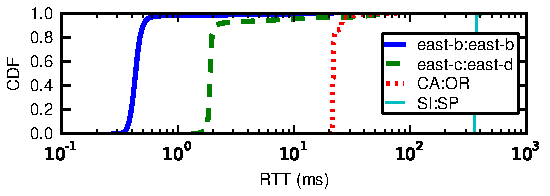
\includegraphics[width=\columnwidth]{graphs/ping-plot.pdf}\vspace{-1em}
\caption{CDF of round-trip times for slowest inter- and intra-
  availability zone links compared to cross-region links.}\vspace{-1em}
\label{fig:rtt}
\end{figure}

In real deployments, messages travel slower than the speed of light
due to routing, congestion, and server-side overheads. To illustrate
the difference between intra-datacenter, inter-datacenter, and
inter-planetary networks, we performed a measurement study of network
behavior on Amazon's EC2, a widely-used public compute cloud. We
measured one week of ping times between all seven EC2 geographic
``regions'', across three ``availability zones'' (closely co-located
datacenters), and within a single ``availabilty zone'' (datacenter),
at a granularity of 1s (dataset to be released). We summarize the
results of our network measurement study in Table~\ref{table:rtt}. On
average, intra-datacenter communication (Table 1a) is between 1.82 and
6.38 times faster than across geographically co-located datacenters
(Table 1b) and between 40 and 647 times faster than across
geographically distributed datacenters (Table 1c). The cost of
wide-area communication exceeds the speed of light: for example, while
a speed-of-light RTT from S\~{a}o Paulo to Singapore RTT is 106.7ms,
ICMP packets incur an average 362.8ms RTT (95th percentile: 649ms). As
shown in Figure~\ref{fig:rtt}, the distribution of latencies varies
between links, but the trend is clear: remote communication has a
substantial cost.

\section{When is ``ACID'' ACID?}
\label{sec:modernacid}

The previous section demonstrated that distributed systems must
address partitions and latency: what does this mean for distributed
databases? Database researchers and designers have long realized that
serializability is not achievable in a highly available
system~\cite{davidson-survey}, meaning that, in environments like
those in Section~\ref{sec:motivation}, database designs face a choice
between availability and strong semantics. However, even in a
single-node database, the coordination penalties associated with
serializability can be severe, manifesting themselves in the form of
decreased concurrency (and, subsequently, performance degradation,
scalability limitations, and, often, external aborts like
deadlocks)~\cite{gray-isolation}. Accordingly, to increase
concurrency, database systems offer a range of ACID properties weaker
than serializability.  Instead, databases offer a host of so-called
\textit{weak isolation} models that allow varying restrictions on the
space of schedules that are allowable by the system~\cite{adya,
  ansicritique, ansi-sql}. None of these weak isolation models
guarantees serializability, but, as we see below, their benefits are
often considered to outweigh costs of possible consistency anomalies
that might arise from their use.

To understand the prevalence of these weak isolation models, we
recently surveyed the default and maximum isolation models provided by
18 databases, often claiming to provide ``ACID'' or ``NewSQL''
functionality~\cite{hat-hotos}. As shown in
Table~\ref{table:existing}, only three out of 18 databases provided
serializability by default, and eight did not provide serializability
as an option at all. This is particularly surprising when we consider
the widespread deployment of many of these non-serializable databases,
like Oracle 11g, which are known to power major businesses and product
functionality. Given that these transactional models are frequently
used, our inability to provide serializability in arbitrary HATs
appears non-fatal for practical applications. If application writers
and database vendors have already decided that the benefits of weak
isolation outweigh potential application inconsistencies, then, in a
highly available environment that prohibits serializability, similar
decisions may be tenable.

\begin{table}
\begin{center}
\begin{small}
\begin{tabular}{|l|c|c|}
\hline
Database & Default & Maximum\\\hline
Actian Ingres 10.0/10S & S & S\\
Aerospike & RC & RC\\
Akiban Persistit & SI & SI\\
Clustrix CLX 4100 & RR & RR\\
Greenplum 4.1 & RC & S \\
IBM DB2 10 for z/OS & CS & S\\
IBM Informix 11.50 & Depends & S\\
MySQL 5.6 & RR & S \\
MemSQL 1b & RC & RC\\
MS SQL Server 2012 & RC & S \\
NuoDB & CR & CR\\
Oracle 11g & RC & SI\\
Oracle Berkeley DB & S & S\\
Oracle Berkeley DB JE & RR & S\\
Postgres 9.2.2 & RC & S\\
SAP HANA & RC & SI\\
ScaleDB 1.02 & RC & RC\\
VoltDB & S & S\\
\hline
\multicolumn{3}{|p{7cm}|}{{\footnotesize RC: read committed, RR: repeatable read, SI: snapshot isolation, S: serializability, CS: cursor stability, CR: consistent read}}\\\hline

\end{tabular}
\caption{Default and maximum isolation levels for ACID and NewSQL
  databases as of January 2013 (from
  \protect\cite{hat-hotos}).}\vspace{-1.5em}
\label{table:existing}
\end{small}
\end{center}
\end{table}

It is unknown \textit{which} of these guarantees can be provided with
high availability. The existing algorithms for providing weak
isolation are typically designed for a single-node context and are, to
the best of our knowledge, unavailable due to a reliance on
concurrency control mechanisms like locking that are not resilient to
partial failure (Section~\ref{sec:evaluation}). Moreover, we are not
aware of any prior literature that provides guidance as to the
relationship between weak isolation and high availability: prior work
has examined the relationship between serializability and high
availability~\cite{davidson-survey} and weak isolation on a single
server~\cite{adya, ansicritique, gray-isolation} but never weak
isolation and high availability taken together.  A primary goal in the
remainder of this paper is to understand which models are
HAT-compliant.

